% LectureTemplate for ME3050 -  Dynamics Modeling and Controls - Tennessee Technological University
% Tristan Hill - Spring 2020 - Summer 2020 - Fall 2022
% Dynamics Modeling and Controls
% Lecture Module - ODE review - Topic 2  - Separation of Variables

% Document settings

%\documentclass{beamer}                  % for presentation ?
\documentclass[handout]{beamer}  % for handout ?

\usepackage{/home/thill/Documents/lectures/dmc_lectures/dmc_lectures}

\newcommand{\TNUM}{2\hspace{2mm}} % Topic number 
\newcommand{\moduletitle}{ODE Review} % Titles and Stuff
\newcommand{\topictitle}{Separation of Variables} 

\newcommand{\sectiontitleI}{Review} % More Titles and Stuff
\newcommand{\sectiontitleII}{Separation of Variables}
\newcommand{\sectiontitleIII}{Example}

\author{ME3050 - Dynamic Modeling and Controls}
\title{Lecture Module - \moduletitle}
\date{Mechanical Engineering\vspc Tennessee Technological University}

\begin{document}
	
	\lstset{language=MATLAB,basicstyle=\ttfamily\small,showstringspaces=false}
	
	\frame{\titlepage \center\begin{framed}\Large \textbf{Topic \TNUM - \topictitle}\end{framed} \vspace{5mm}}
	
	% Section 0 - Outline
	\frame{
		
		\large \textbf{Topic \TNUM - \topictitle} \vspace{3mm}\\
		
		\begin{itemize}
			
			\item \sectiontitleI    \vspc % Section I
			\item \sectiontitleII 	\vspc % Section II
			\item \sectiontitleIII 	\vspc %Section III
			
		\end{itemize}
		
	}

\section{\sectiontitleI}

\frame{

  \frametitle{What is a Differential Equation? Solution?}

A {\bf differential equation} is an equation which describes a function \vspace{3mm}\\and one or more of its \underline{\hspace{50mm}} of the \vspace{3mm}\\ \underline{\hspace{50mm}}\hspace{3mm}\underline{\hspace{50mm}}\vspace{2mm}\\ with respect to the \underline{\hspace{60mm}}. \vspace{8mm} \\
 
The {\bf solution} to a differential equation describes the \vspace{2mm}\\ \underline{\hspace{40mm}}\hspace{2mm}\underline{\hspace{40mm}} as a function \vspace{2mm}\\of the \underline{\hspace{40mm}}\hspace{2mm}\underline{\hspace{40mm}}.  \vspace{5mm}\\

}

\section{\sectiontitleII}
%\subsection{Problem Statement}
\frame{

\frametitle{Problem Statement}



Remember our example from the previous lecture?\vspace{5mm}\\

        \scalebox{1.25}{$\dot{v}+\frac{c}{m}v=f(t)$} \vspace{2mm}\\
	
	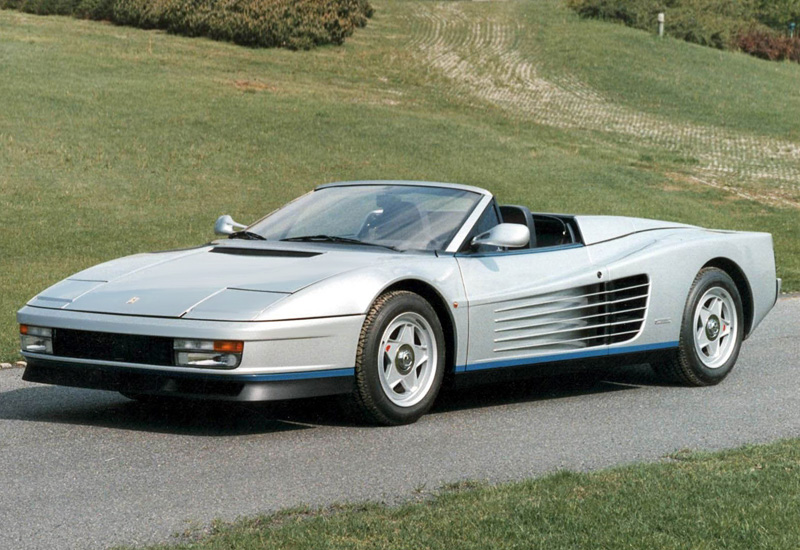
\includegraphics[scale=0.15]{ferrari.jpg} \hspace{10mm} 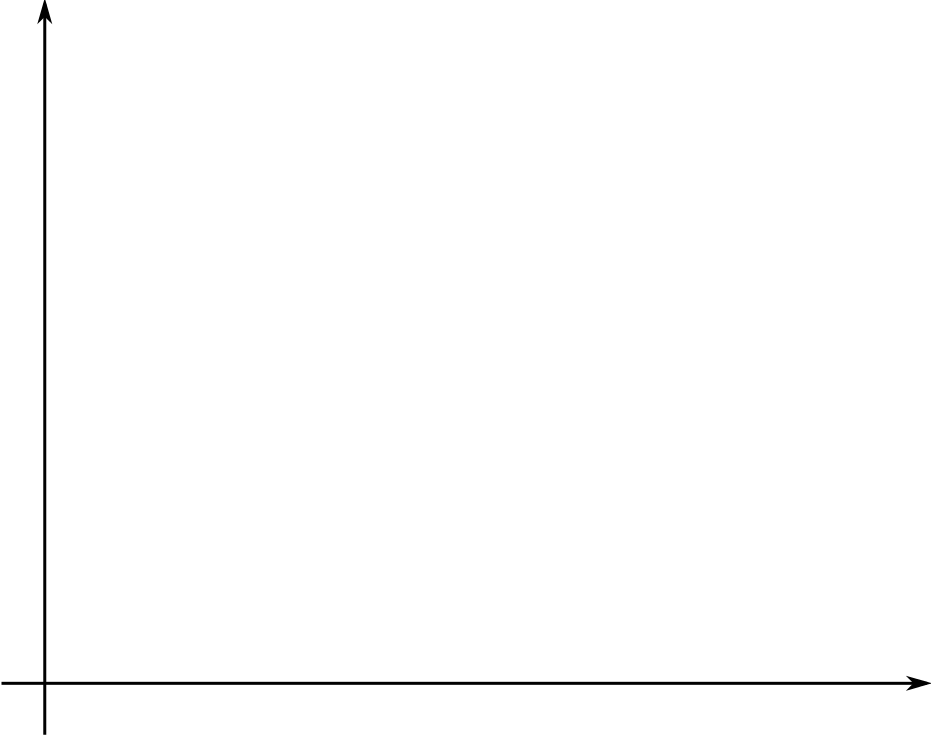
\includegraphics[scale=0.10]{lecture1_fig2.png}\vspace{2mm}\\
	
	
We are going to find an {\bf analytical solution} to this problem. 
  

}

%\subsection{Separation of Variables}
\frame{

\frametitle{Separation of Variables}

This is an {\bf analytical} method that you learned in calculus. \vspace{2mm}\\
Assume the external force $f(t)$ is zero. Re-write then separate. \vspace{5mm}\\

\scalebox{1.25}{$\dot{v}+\frac{c}{m}v=0$} \vspace{50mm}\\

}

%\subsection{Solution}
\frame{

\frametitle{Solution}

The solution $v(t)$ has been found. What does it mean? What do we do next?\vspace{5mm}\\

\scalebox{1.25}{$v(t)=$} \vspace{50mm}\\


}

\frame{

\frametitle{Graph of Solution}

What does the solution look like?\vspace{5mm}\\
\scalebox{1.25}{$v(t)=v_0e^{-\frac{c}{m}t}$} \vspace{5mm}\\

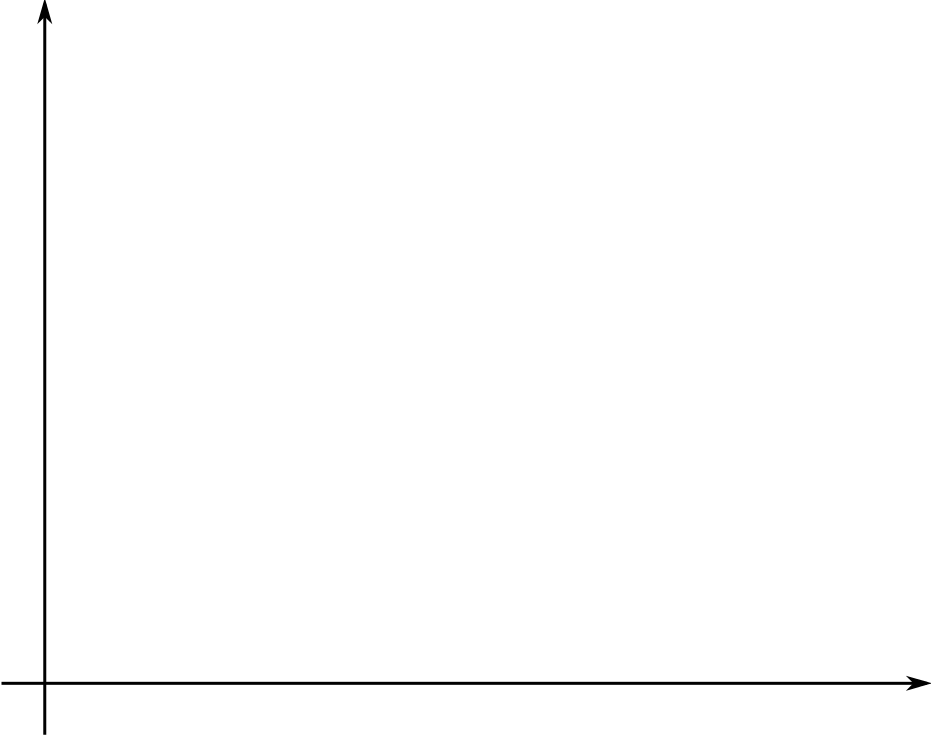
\includegraphics[scale=0.15]{lecture1_fig2.png}\hspace{5mm}%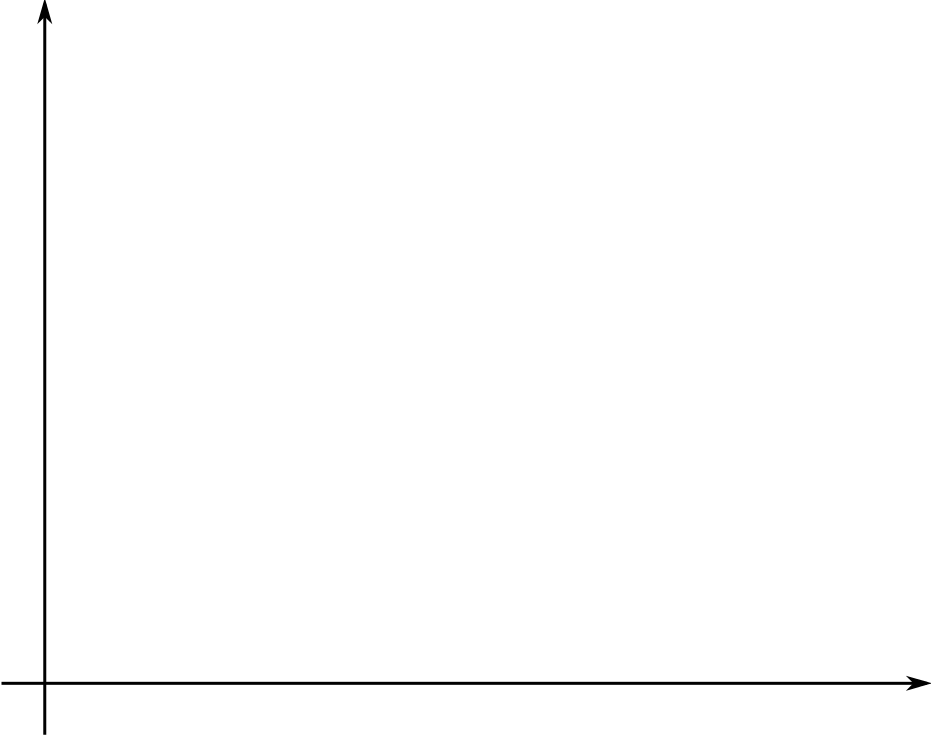
\includegraphics[scale=0.15]{lecture1_fig2.png}

}


\end{document}









